\newif\ifshowsolutions
\showsolutionstrue
\documentclass{article}
\usepackage{listings}
\usepackage{amsmath}
%\usepackage{subfigure}
\usepackage{subfig}
\usepackage{amsthm}
\usepackage{amsmath}
\usepackage{amssymb}
\usepackage{graphicx}
\usepackage{mdwlist}
\usepackage[colorlinks=true]{hyperref}
\usepackage{geometry}
\usepackage{titlesec}
\geometry{margin=1in}
\geometry{headheight=2in}
\geometry{top=2in}
\usepackage{palatino}
\usepackage{mathrsfs}
\usepackage{fancyhdr}
\usepackage{paralist}
\usepackage{todonotes}
\setlength{\marginparwidth}{2.15cm}
\usepackage{tikz}
\usetikzlibrary{positioning,shapes,backgrounds}
\usepackage{float} % Place figures where you ACTUALLY want it
\usepackage{comment} % a hack to toggle sections
\usepackage{ifthen}
\usepackage{mdframed}
\usepackage{verbatim}
\usepackage[strings]{underscore}
\usepackage{listings}
\usepackage{bbm}
\rhead{}
\lhead{}

\renewcommand{\baselinestretch}{1.15}

% Shortcuts for commonly used operators
\newcommand{\E}{\mathbb{E}}
\newcommand{\Var}{\operatorname{Var}}
\newcommand{\Cov}{\operatorname{Cov}}
\newcommand{\Bias}{\operatorname{Bias}}
\DeclareMathOperator{\argmin}{arg\,min}
\DeclareMathOperator{\argmax}{arg\,max}

% do not number subsection and below
\setcounter{secnumdepth}{1}

% custom format subsection
\titleformat*{\subsection}{\large\bfseries}

% set up the \question shortcut
\newcounter{question}[section]
\newenvironment{question}[1][]
  {\refstepcounter{question}\par\addvspace{1em}\textbf{Question~\Alph{question}\!
    \ifthenelse{\equal{#1}{}}{}{ [#1 points]}: }}
    {\par\vspace{\baselineskip}}

\newcounter{subquestion}[question]
\newenvironment{subquestion}[1][]
  {\refstepcounter{subquestion}\par\medskip\textbf{\roman{subquestion}.\!
    \ifthenelse{\equal{#1}{}}{}{ [#1 points]:}} }
  {\par\addvspace{\baselineskip}}

\titlespacing\section{0pt}{12pt plus 2pt minus 2pt}{0pt plus 2pt minus 2pt}
\titlespacing\subsection{0pt}{12pt plus 4pt minus 2pt}{0pt plus 2pt minus 2pt}
\titlespacing\subsubsection{0pt}{12pt plus 4pt minus 2pt}{0pt plus 2pt minus 2pt}


\newenvironment{hint}[1][]
  {\begin{em}\textbf{Hint: }}{\end{em}}

\ifshowsolutions
  \newenvironment{solution}[1][]
    {\par\medskip \begin{mdframed}\textbf{Solution~\Alph{question}#1:} \begin{em}}
    {\end{em}\medskip\end{mdframed}\medskip}
  \newenvironment{subsolution}[1][]
    {\par\medskip \begin{mdframed}\textbf{Solution~\Alph{question}#1.\roman{subquestion}:} \begin{em}}
    {\end{em}\medskip\end{mdframed}\medskip}
\else
  \excludecomment{solution}
  \excludecomment{subsolution}
\fi

\newcommand{\boldline}[1]{\underline{\textbf{#1}}}

% User packages
\usepackage[labelfont=bf]{caption}
\usepackage[labelfont=bf]{caption}
\usepackage[labelfont=bf]{caption}
\usepackage [english]{babel}
\usepackage [autostyle, english = american]{csquotes}
\MakeOuterQuote{"}

% User commands
\setlength{\parindent}{0pt}

\chead{%
  {\vbox{%
      \vspace{2mm}
      \large
      Machine Learning \& Data Mining \hfill
      Caltech CS/CNS/EE 155 \hfill \\[1pt]
      Miniproject 1\hfill
      Released January $28^{th}$, 2017 \\
    }
  }
}

\begin{document}
\pagestyle{fancy}

\section*{1. Introduction}
\medskip
\begin{itemize}

    \item \boldline{Group members} \\
    Eli Sorey \\
    Kun ho (John) Kim

    \item \boldline{Team name} \\
    Stochastic Gradient, Decent

    \item \boldline{Division of labour} \\
    Eli focused on feature engineering in terms of dataset cleaning, feature selection, and feature transformation. (Feature Engineering) Kun ho primarily worked on the model
    selection, model parameter optimization, and ensemble selection methods. (Models and techniques) We delve into the specific of our work in the following sections.

\end{itemize}



\section*{2. Overview}
\medskip
\begin{itemize}

    \item \boldline{Models and techniques tried}
    \begin{itemize}
    \item \textbf{*Ensemble Selection:} Submitted model.
    \item \textbf{Gradient Boosting Machines:}
    \item \textbf{Random Forest:}
    \item \textbf{Adaptive Boosting:}
    \item \textbf{Extra Trees:}
    \item \textbf{Support Vector Machines:}
    \item \textbf{Artificial Neural Networks:}
    \end{itemize}

    \item \boldline{Work timeline}
    \begin{itemize}
    \item \textbf{Day1 - Day4:} Preliminary data-processing \& Broad model selection.
    \item \textbf{Day 4 - Day 8:} Feature engineering \& Single model optimization
    \item \textbf{Day 8 - Day 12:} Ensemble selection \& Final model tuning
    \end{itemize}

\end{itemize}


\newpage


\section*{3. Approach \& Results}
\subsection*{3.1. Overview}
Our team's general pipeline for this competition is outlined in the flow chart below. \\
\begin{figure}[h]
\center
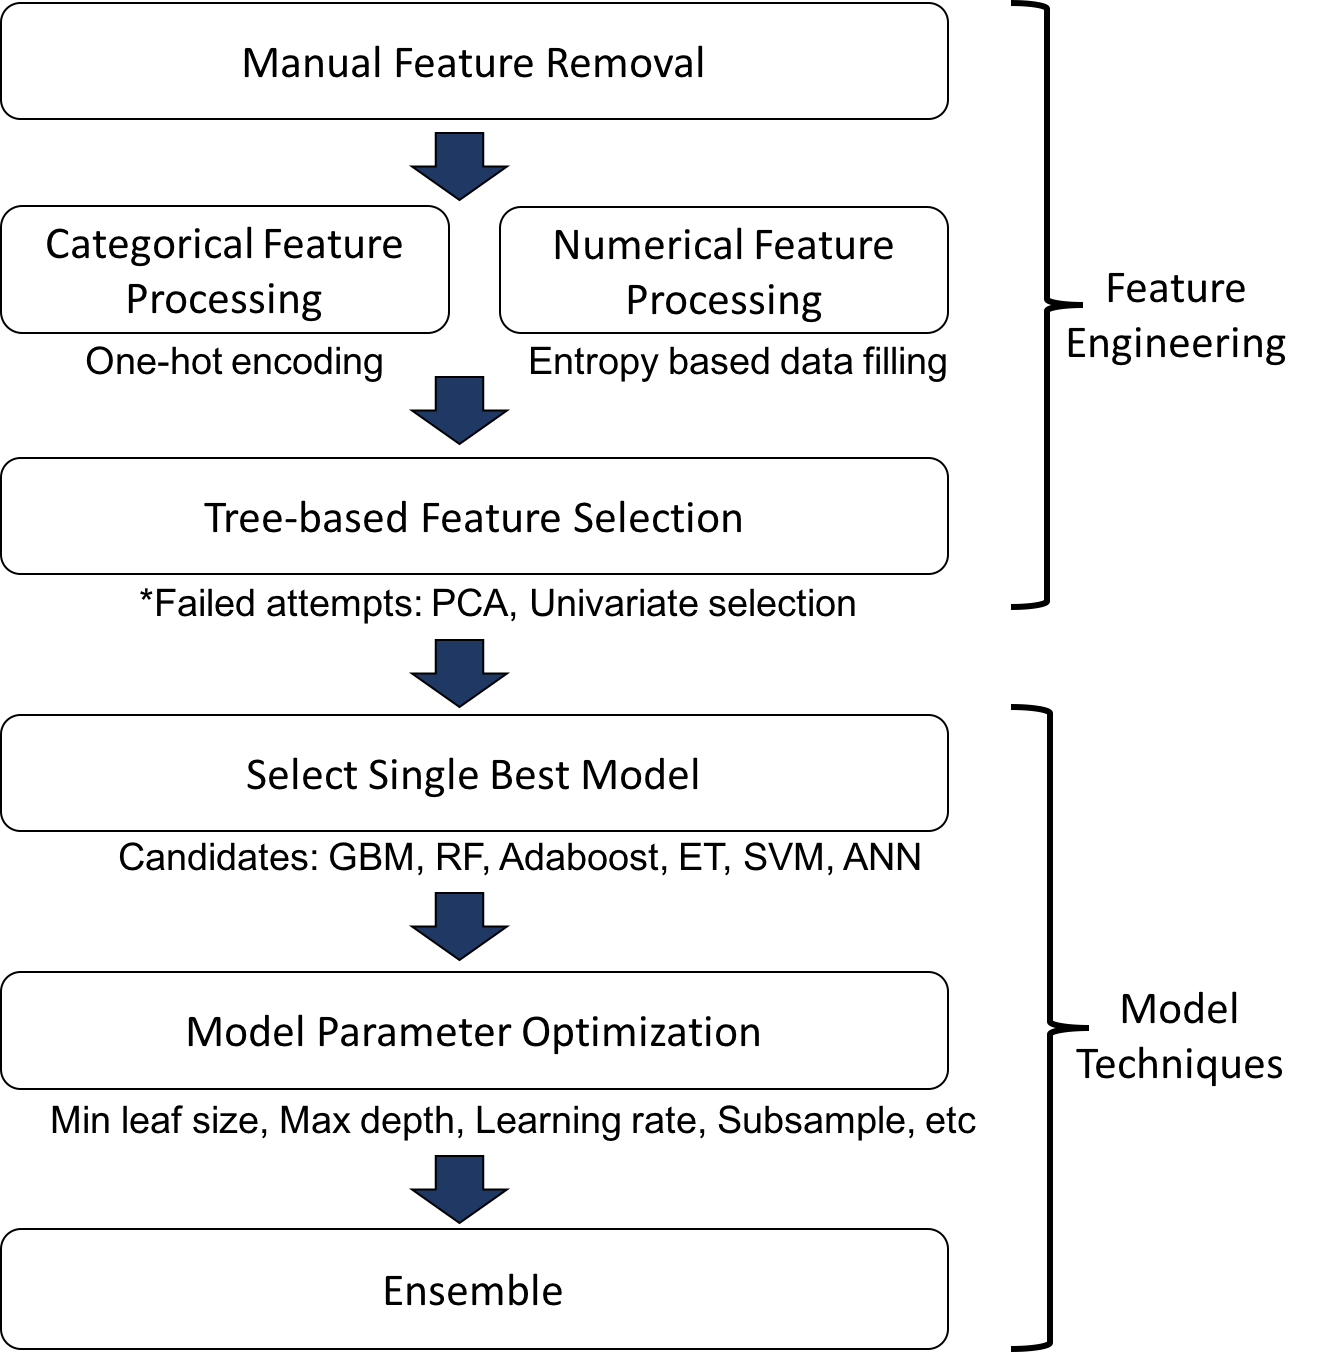
\includegraphics[scale=0.4]{figure1/figure1.png}
\caption{\textbf{Overall pipeline}}
\end{figure}

We first sought to transform the raw training data into a compact representation while keeping all the relevant information. The feature engineering part of the workflow covers methods of handling categorical features, numerical features, and the feature selection process. The model \& techniques part covers our methods of model selection, parameter
optimization, and stacking/ensemble selecting single models.

\subsection*{3.2. Feature engineering}
The philosophy guiding our approach to feature engineering was to make it as straightforward as possible for our models to pick up on the structures in the data. To this end, we sought to remove low-signal features and to reformat other features to be more accessible to our models. The first step in this process was to familiarize ourselves with the data. This was accomplished by reading through the 2008 Codebook describing each of the features. One thing that immediately stood out was the presence of several classes of features that would not be useful to our predictive models. For example,  104 features were marked as 'allocation flags'. Each of these features is associated with another feature, and indicates whether or not the survey participant modified his/her original response. These features were dropped because they do not help in our prediction problem. Other classes of features that were dropped included recodes (redundant features), features that only attained one value on the training set, and features which had responses on less than 1\% of the training set.\\

Once these unhelpful features were trimmed off of the data, we began looking at ways to make the remaining features more useful to our models. One recurring theme was the presence of features that were numerical encodings of categorical values. For instance, the feature 'PEIO1ICD' was a code for the survey participant's primary occupational industry. Values for this feature ranged from -9 to 9890. It was obvious that this feature had the potential to be predictive, but in its original form, it risked being confusing to our models. This is because a value of 5000 should not be interpreted to be "5 times higher" than a value of 1000; they are simply different categories. To get around this, we converted all such features into categorical flag features. To do this, we first mapped the encoded values to their categories (a value of 7970 for 'PEIO1ICD' became 'healthcare service', for instance), and then used the Pandas library to create a new feature for each of the categorical values attained by the original feature. These new features took on value 0 for all participants who did not belong to that category, and value 1 for all those who did. The original columns were then dropped. We found that this processing improved the performance of our models, both on the validation sets and on the test set.

We also spent time thinking about how best to deal with negative values. As outlined in the codebook, negative values coincide with nonresponses of various kinds. For instance, -1 means that the participant left this question blank, and -3 means the participant refused to answer the question. A standard approach to this issue is to replace the nonreponses with the mean of the nonnegative values attained by the feature of interest. Our concern was that doing this may mislead the prediction model, particularly if the feature carried a high degree of importance for the model. One way in which we attempted to avoid this issue is the following. Given a feature, we first computed the possible splits that a decision tree could possibly make. We then found the split that minimized the entropy, corresponding to the choice of split a decision tree would make. Finally, we found the mean of the \textit{higher} entropy side of the split, and used that as our fill value for nonresponses within that feature. The logic behind this is that we wanted the fill value to contribute as little as possible to the model's eventual prediction. By using the maximum entropy side, we gave the model as little information as possible through the fill value. Unfortunately, this approach led to decreased model performance, and we reverted to the simple plan of using the mean of the feature.\\

The transformations described above ultimately yielded a training set with ~1600 features. At this point, we opted to trim down the number of features before training our models, in the process of feature selection. To do this, we trained an ExtraTreesClassifier from sci-kit learn on the transformed data, and then sorted the features by their importance within the trained model. We then took those features whose importances were greater than some fixed constant times the mean of the importances. Our goal was to select between 100 and 300 features from the data. Depending on the exact details of our previous feature engineering, the fixed constant was between 1.0 and 3.5.\\

At this point, our data was ready to be handed to the models for training.

\newpage

\subsection*{3.3. Model \& Techniques}
\subsubsection*{[i]. Single model selection through cross validation}
Once we we obtained a compact representation of the raw data, 6 general model classes(GBM, RF, Adaboost, ET, SVM, ANN) were considered as candidates to determine which attains the best single-model performance. 5-fold cross validation was performed and the model with the highest validation accuracy was chosen as the best model. The following bar graph demonstrates that gradient boosting machines (GBM) performed the best with a validation accuracy of $78.4\%$.
\begin{figure}[h]
\center
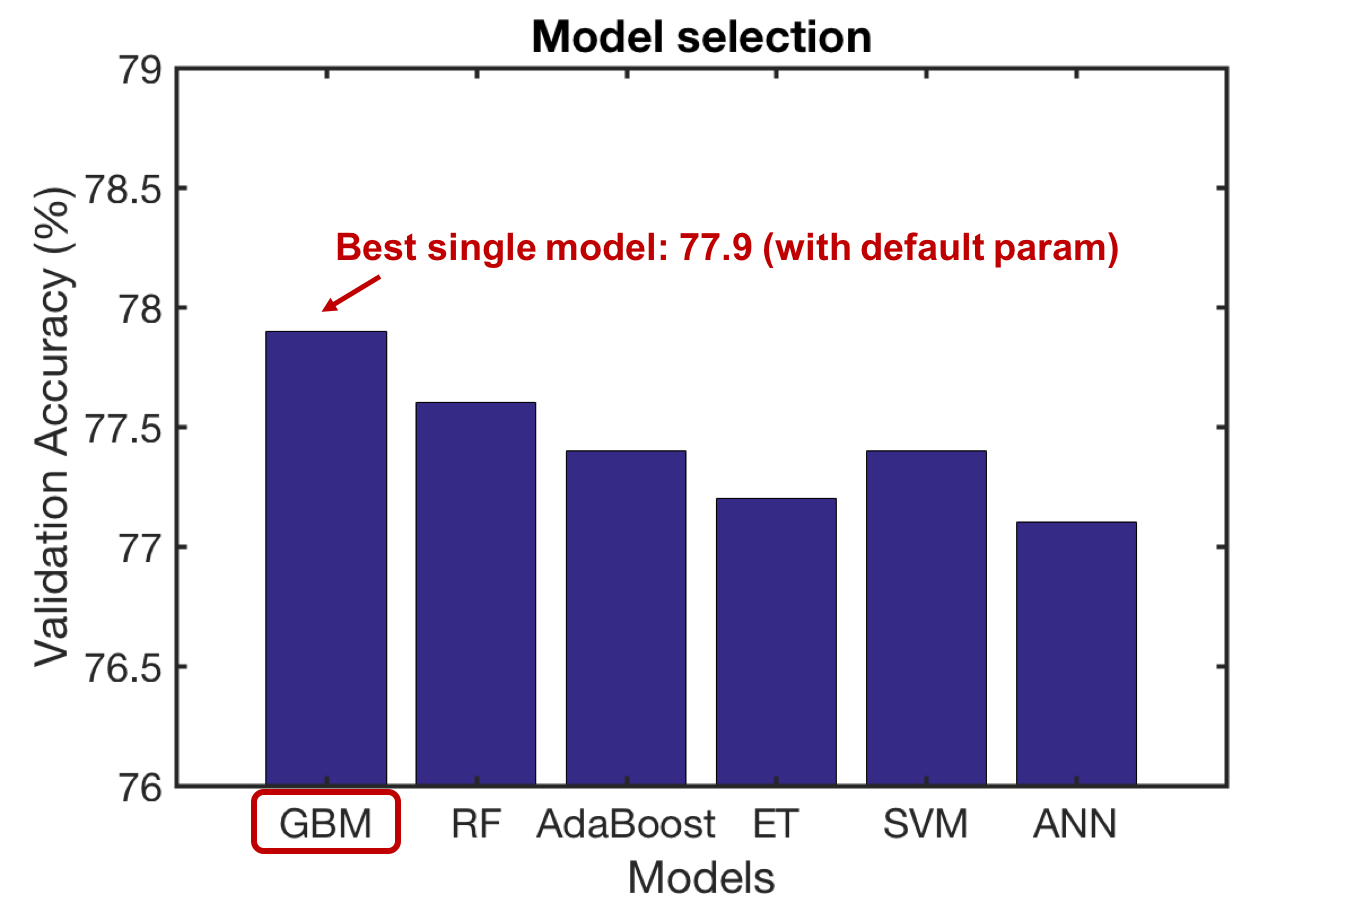
\includegraphics[scale=0.45]{figure2/figure2.png}
\caption{\textbf{Cross validation for model class selection} \textit{GBM attains the highest accuracy of $78.4\%$ followed by random forests(77.6), Adaboost(77.4), Extra Trees(77.2), Support Vector Machines (77.4), and Artificial Neural Networks (77.1).}}
\end{figure}

Generally, we saw that tree-based non-linear classifiers out-performed linear models such as support vector machines. We attribute this to the fact that demographic can be highly non-linear. This is in agreement with the fact that the training data projected onto the first two principal components showed no notable separating boundaries during the PCA analysis. This influenced our decision of including more tree-based non-linear classifiers into the pool of models to perform cross validation on. One notable discovery that we made was that gradient boosting machines provide stable performance in the sense that there's not much stochasticity in the validation accuracy when we train over the same data. This low-variance can be attributed to the nature of boosting methods, which train several decision trees. However, the low variance characteristic made it difficult to enhance the performance of GBMs by only including GBMs in the pool of trained models to select on. Section 3.3-[iii] will elaborate more on this issue.

\newpage

\subsubsection*{[ii]. Parameter optimization for GBM}
We considered 4 main parameters for optimization: minimum leaf size, maximum height, learning rate, subsample.

\newpage
\subsubsection*{[iii]. Handling class-imbalance}
Upon analyzing the label distribution of the training data, we found that over $73\%$ were of class $1$, while only $27\%$ were class 2. Such class-imbalance can often lead to the tree predicting in favor of the majority class, which generates a low-precision, high-recall classifier. (In terms of the majority class) Our solution to tackling this class-imbalance problem was to set a modified threshold for predictions. A decision tree makes predictions by taking the argmax of the probability distribution over the class-labels at each leaf node. For a binary classification task, this means that the class with probability higher than 0.5 becomes the predicted value at a leaf node. We varied the threshold probability that class $1$ had to be in order to be selected as the prediction from $0.498 - 0.502$ and discovered that an optimum threshold exists which maximizes the validation accuracy.

\begin{figure}[h]
\center
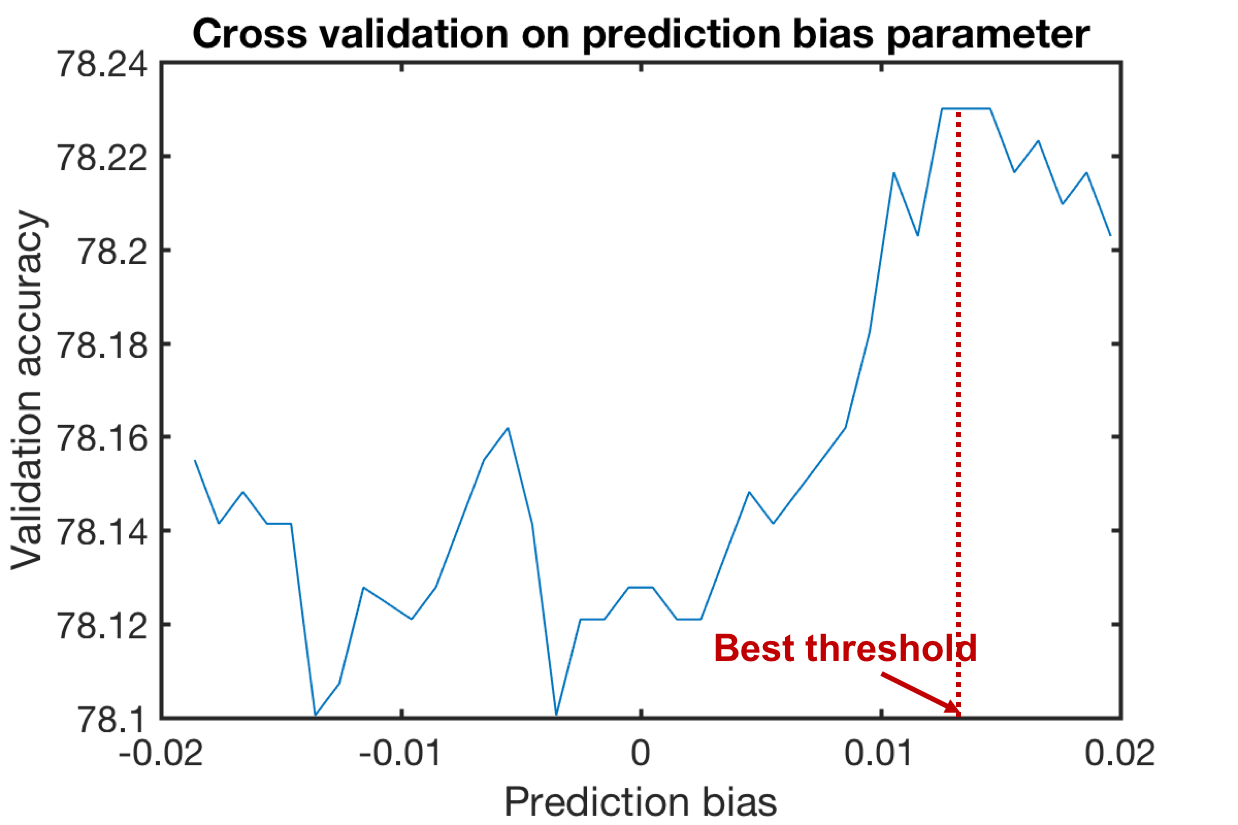
\includegraphics[scale=0.45]{figure4/figure4.png}
\caption{\textbf{Cross validation for model class selection} \textit{GBM attains the highest accuracy of $78.4\%$ followed by random forests(77.6), Adaboost(77.4), Extra Trees(77.2), Support Vector Machines (77.4), and Artificial Neural Networks (77.1).}}
\end{figure}

\newpage

\section*{4. Discussion}
\medskip
\begin{itemize}

    \item \boldline{Scoring} \\
    % Insert text here.

    \item \boldline{Validation and Test} \\
    % Insert text here.

\end{itemize}



\section*{5. Conclusion}
\medskip
\begin{itemize}

    \item \boldline{Discoveries} \\
    % Insert text here.

    \item \boldline{Challenges} \\
    It was difficult to decide what to do with the various nonresponse values (negative values), as described in Section 3.2. Ensuring that the transformed training data and test data were compatible (ie, had the same shape) was an issue because our handling of categorical features sometimes created discrepancies in the number of features between the training and test sets. For instance, that a categorical feature attains values 1 and 2 in the training set and 3 in the test set. Then the transformed training set will have two features for the original categorical feature, whereas the transformed test set will have only one. This was remedied by adding additional feature columns to both data sets to ensure that they had the same features.

    \item \boldline{Concluding Remarks} \\
    % Insert text here.

\end{itemize}



\end{document}
